\documentclass{article}
\usepackage{hyperref}
\usepackage{graphicx}\usepackage{AOcommon}
% \usepackage{makeidx}
\usepackage{listings}\lstset{
    language=Java,
    basicstyle=\scriptsize,
    breaklines=true,
    tabsize=4,}
\def\auxilliaries{}

\title{\fmas -- A Flexible and Lightweight \\ Agent Shell}
\author{}
\date{\today}

\begin{document}\maketitle

\tableofcontents\clearpage

\section{Concepts and terminology}
\begin{itemize}
    \item agent
    \item entity
    \item deployment
    \item message
    \item context
\end{itemize}

\section{Functionality}

\clearpage
\subsection{Hello World -- A simple Java agent}

Writing a new agent in \fmas is as simple as extending the \code{BaseAgent} class and overriding the \code{start()} method. Extending \code{BaseAgent} is not mandatory, but implementing the \code{Agent} interface would require implementing more methods, as described in section \todo{ref section entities / EntityBase}.

\begin{figure}[ht]\centering
\begin{lstlisting}
import net.xqhs.flash.core.agent.BaseAgent;

public class HelloWorldAgent extends BaseAgent {
	public boolean start() {
		if(!super.start()) return false;
		li("Hello World");
		stop();
		return true;
	}
}
\end{lstlisting}
\caption{Hello World agent.}\label{fig:func:helloWorld:code}
\end{figure}

The code for the Hello World agent is shown in Figure \ref{fig:func:helloWorld:code}. The implementation uses the \code{li} method for logging, a mechanism which is detailed in section \todo{ref Logging}, but it could have used \code{System.out.println()} just the same.

The Hello World example agent is implemented in package \code{src-examples/example}.

For deploying the Hello World agent, one could use one of two possibilities of configuring a deployment (more details on configuring deployments, or deploying without a configuration, in Section \todo{ref deployment configuration}): via command line arguments or via an XML deployment file. These two manners of creating a deployment are illustrated in the classes \code{BootDeployment} and \code{BootCLI} in the same package as the Hello World agent.

\todo{document usage using the \fmas jar, not the repository itself}
\todo{mention generating of lib-all if using the sources}

To start the deployment directly from the system terminal, in the root of the repository, one can run, for the two variants, respectively\footnote{In Windows, semi-colon must be used instead of a colon in the value for \code{-cp}.}:

\begin{lstlisting}[language=bash]
    java -cp "bin:lib-all/*" quick.Boot -agent HelloWorldAgent classpath:example.helloWorld.HelloWorldAgent
\end{lstlisting}

\begin{lstlisting}[language=bash]
    java -cp "bin:lib-all/*" quick.Boot src-examples/example/helloWorld/deployment.xml
\end{lstlisting}

\clearpage
\subsection{Configuring entities}


\begin{figure}[t]\centering
\begin{lstlisting}
import net.xqhs.flash.core.agent.BaseAgent;

public class ConfigurableHelloWorldAgent extends BaseAgent {

    public boolean start() {
        if (!super.start()) return false;

        Timer t = new Timer();
        t.schedule(new TimerTask() {
            @Override
            public void run() {
                stop();
                t.cancel();
            }
        }, stopAfter);

        return true;
    }
}
\end{lstlisting}
\caption{Configurable Hello World agent.}\label{fig:func:configurableHelloWorldGeneral:code}
\end{figure}

The Agent Configuration example is implemented in package \code{src-examples/example}. The difference between the Agent Configuration example and the previous one is the implementation of the overridden \code{start()} method.

The code for the Configurable Hello World agent is shown in Figure \ref{fig:func:configurableHelloWorldGeneral:code}. The implementation uses the \code{stopAfter} parameter and \code{Timer} class to schedule when the agent should stop. We will now present in detail how parameters for an entity can be configured in the deployment and how they can be extracted by the entity from that configuration.

The parameters of an entity can be \emph{sent} via the following two variants:
\begin{itemize}
    \item in a deployment configured via the command line. Figure~\ref{fig:configFigure} presents the configuration needed to start the deployment via command line arguments: the name of the agent, classpath and \code{stopAfter} parameters.
    \item in a deployment configured in an XML deployment file. Figure~\ref{fig:func:deploymentXMLFile:code} presents the parameters needed to start a deployment via XML deployment file, being the same as above.
\end{itemize}


\begin{figure}[t]
\centering
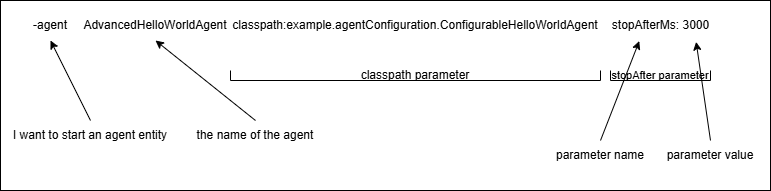
\includegraphics[width=\tw]{../img/config-figure.png}
  \caption{Configuration of parameters of an entity via command line arguments.}
  \label{fig:configFigure}
\end{figure}



The Configurable Hello World agent is implemented in two variants, the difference being how the parameters are extracted from the configuration, presented below.

% The deployment of the Configurable Hello World agent is performed in two variants, as presented in the simple Java agent.


\begin{figure}[ht]\centering
\begin{lstlisting}
<deployment>
    <agent classpath="example.agentConfiguration.ConfigurableHelloWorldAgent" name="HelloWorldAgent">
        <parameter name="stopAfterMs" value="3000"/>
    </agent>
</deployment>
\end{lstlisting}
\caption{Configuration of parameters of an entity via XML deployment file.}\label{fig:func:deploymentXMLFile:code}
\end{figure}

There are also two variants through which the parameters received in the configuration can be extracted by an entity:
\begin{itemize}
    \item extending the \code{EntityCore} class and using the \code{getConfiguration()} method. Figure~\ref{fig:func:ConfigurableHelloWorldAgent1:code} presents the code in this scenario. The implementation uses the \code{getConfiguration()} method for extracting \code{stopAfter} parameter.
    \item overriding the \code{configure()} method. Figure~\ref{fig:func:ConfigurableHelloWorldAgent2:code} presents the code in this scenario. The implementation overrides the \code{configure()} method and extracts the \code{stopAfter} parameter. The \code{configure()} method of an entity is called immediately after its construction.
\end{itemize}

\begin{figure}[ht]\centering
\begin{lstlisting}
public class ConfigurableHelloWorldAgent extends BaseAgent {

	public boolean start() {
		if(!super.start()) return false;
		
		long stopAfter = getConfiguration().get(STOP_AFTER_PARAMETER_NAME)).orElse(DEFAULT_STOP_AFTER);
		
		Timer t = new Timer();
		t.schedule(new TimerTask() {...}, stopAfter);
		return true;
	}
}
\end{lstlisting}
\caption{Configurable Hello World Agent extending \code{EntityCore} class and using \code{getConfiguration()} method.}\label{fig:func:ConfigurableHelloWorldAgent1:code}
\end{figure}


\begin{figure}[ht]\centering
\begin{lstlisting}
public class ConfigurableHelloWorldAgent2 extends BaseAgent {

	@Override
	public boolean configure(MultiTreeMap configuration) {
		if(configuration.isSet(STOP_AFTER_PARAMETER_NAME))
			stopAfter = configuration.getFirstValue(STOP_AFTER_PARAMETER_NAME);
		else
			stopAfter = DEFAULT_STOP_AFTER;
		return true;
	}
}
\end{lstlisting}
\caption{Configurable Hello World Agent implementing \code{configure()} method.}\label{fig:func:ConfigurableHelloWorldAgent2:code}
\end{figure}

It can be observed that the \code{configure()} method receives, as parameter, the configuration, as a \code{MultiTreeMap} object. The \code{getConfiguration()} method returns an object of the same type.

The \code{MultiTreeMap} class acts as a tree of key-value pairs that allows multiple values for the same key. Keys are also called names.
The class builds on the same principles as the \code{MultiValueMap} but acts rather like a hierarchical \code{MultiValueMap}. It has two types of names.
Some names are "simple", in that they act exactly like names with String values in the \code{MultiValueMap}. There is a name and one or more String values associated with the name.
Other names are "hierarchical" (or tree-keys). Each hierarchical name has one or more associated \code{MultiTreeMap} values.
The class extends the \code{MultiValueMap} such that only the two types of values are admitted: String and the \code{MultiTreeMap}. One name can be associated either with String values, or with tree values, but not with a combination thereof (a name must either be simple or hierarchical).
There is no intersection allowed between the set of names for simple values and the set of types for tree values.
For clearer implementation and easier debugging, there are separate methods for the names which are supposed to only hold one value (call them singleton names), both for simple and for tree names. It is possible to change the singleton status of names by calling makeSingleton.


\clearpage
\subsection{Transmission of messages between entities}\label{sec:functionality:messages}

Several examples of message transmission are implemented in subpackages of \code{src-examples/example}. In all of them, the scenario is of two or more agents which send ping-pong messages between them. Ping agent sends a ping every one second to the pong agent and the pong agent replies with a "pong" message to the ping agent. This process ends when the predefined limit has been reached. % The scenario is given as console arguments.

\subsubsection{\emph{Waves}}\label{sec:functionality:messages:waves}


In \fmas[], an interaction between entities is performed via a \emph{wave}, implemented in the class \code{AgentWave}. 

Figure~\ref{fig:functionality:messages:waves:AgentWaveClassDiagram2} presents the class diagram of \code{AgentWave} in which the most important methods were included.

\begin{figure}[t]
\centering
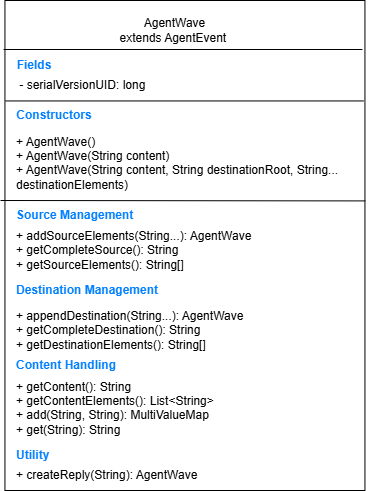
\includegraphics[scale=0.6]{../img/AgentWaveClassDiagram2.png}
  \caption{\code{AgentWave} Class Diagram in which the most important methods were included.}
  \label{fig:functionality:messages:waves:AgentWaveClassDiagram2}
\end{figure}

A wave has a \emph{source}, a \emph{destination}, and \emph{content}. Waves are transmitted between entities either directly (via method calling) or by means of a communication infrastructure, which can transmit waves inside the same node or between different nodes.

The source and destination are \emph{endpoints}.
%   and endpoint looks like
An endpoint is represented as a path made of multiple \emph{elements}, separated by the character \code{/}. For example, an endpoint could look like \code{node1/agentA}, including the node name and the agent names, but the elements included in an endpoint before an agent (or, in general, entity) name depend strongly on the communication infrastructure used.

A simple \code{AgentWave} can be created using its default constructor, or with content and the elements in the destination, e.g.:
\begin{lstlisting}
AgentWave wave = new AgentWave("hello", "node1", "agentA");
\end{lstlisting}

The source and destination of a wave can be configured either as full addresses (called \emph{complete} source/destination) or incrementally, using individual elements (called source/destination \emph{elements}). There are methods in the \code{AgentWave} class for \begin{itemize}
    \item element-wise source management: \code{addSourceElements()}, \code{getCompleteSource()}, \code{getSourceElements()}
    \item element-wise destination management \code{appendDestination()},
    \code{getCompleteDestination()}, \code{getDestinationElements()}
    \item computing or resetting the complete source / destination endpoints: \code{createReply()}, \code{makePath()}, \code{pathToElements()}
\end{itemize}

To add content to a wave, one can use the \code{add()} method or provide it through the constructor. Since \code{AgentWave} extends \code{MultiValueMap}, it supports multiple key-value pairs for content. By default, content is associated with the ``content'' key\footnote{Stored as a string in the \code{AgentWave.CONTENT} constant}, but other content keys can be added via \code{add()}. The method \code{getContentElements()} returns all content-related keys, except those used internally for routing.

A \emph{message} is a wave sent between two agents, via a communication infrastructure.
A \emph{Pylon} is an \emph{embodiment} of a communication infrastructure on a node.
Interaction with a communication infrastructure is done directly (via proxy to the pylon) or via a \emph{messaging shard}, which may be custom for the pylon implementation.

% Entities exist in the context of one another. Agents and other entities execute in the context of a node and, most times, in the context of a pylon.

\subsubsection{Using communication pylons directly}\label{sec:using-pylons-directly}
% example
We take an example in which two instances of the same agent class, \code{AgentPingPongPlain}, communicate back and forth by sending and receiving waves through a pylon, which is accessed by entities via a proxy (the \code{WaveMessagingPylonProxy} class). One instance is configured to act as the "ping" initiator (it has a \code{sendTo} parameter pointing to the other agent’s name), while the other implicitly becomes the "pong" responder (it has no \code{sendTo} parameter).


\paragraph{Initialization}

The agent is placed (using information from the deployment configuration) in the context of the pylon. The pylon is visible by the agent via a proxy.
When added in the context of the pylon, the agent \emph{registers} to the pylon -- <what it means to be registered -- the communication infrastructure knows the node where the agent is located and the name of the agent, so it can receive messages>; agent must provide a proxy to the pylon, as a \code{WaveReceiver} instance.

Figure~\ref{fig:func:initialization:code} presents the essential code for the initialization stage. The complete implementation can be seen in the \code{AgentPingPongPlain} class.

\begin{figure}[ht]\centering
\begin{lstlisting}
@Override
public boolean addContext(EntityProxy<Pylon> context) {
    pylonProxy = (WaveMessagingPylonProxy) context;
    return pylonProxy.register(getName(), new WaveReceiver() {
	   @Override
	   public void receive(AgentWave wave) {
		   processEvent(wave);
	   }
    })
}
\end{lstlisting}
\caption{The essential code for the initialization stage}\label{fig:func:initialization:code}
\end{figure}

\paragraph{Sending messages}

The \code{AgentPingPongPlain} agent sends waves periodically using a timer. When the agent starts and it has a list of destinations, it schedules a task that sends a message to each destination every second. Each message contains a ping count and optionally the keyword \code{last} when the limit has been reached. The messages are constructed using the \code{AgentWave} class and sent via the \code{WaveMessagingPylonProxy}. 

Figure~\ref{fig:func:sendPing:code} presents the essential code for the sending messages stage. The complete implementation can be seen in the \code{AgentPingPongPlain} class.

\begin{figure}[ht]\centering
\begin{lstlisting}
protected void sendPing() {
    AgentWave wave = new AgentWave("ping-no " + tick, otherAgent, "pong");
    pylonProxy.send(wave);
}
\end{lstlisting}
\caption{The essential code for the sending messages stage}\label{fig:func:sendPing:code}
\end{figure}


\paragraph{Receiving messages} 

When an \code{AgentPingPongPlain} agent is registered to the pylon, it provides a receiver implementation that is triggered on incoming waves. Upon receiving a wave, the agent inspects its content and, if it is a pong agent -- it was not initialized with a list of agents to ping -- it constructs and sends a reply. Replies use the \code{createReply()} method, which sets the destination to the original source of the message. If the received message contains the keyword \code{last}, the agent stops after replying.

Figure~\ref{fig:func:processEvent:code} presents the essential code for the receiving messages stage. The complete implementation can be seen in the \code{AgentPingPongPlain} class.

\begin{figure}[ht]\centering
\begin{lstlisting}
protected boolean processEvent(AgentWave wave) {
    String replyContent = wave.getContent() + " reply";
    return send(wave.createReply(replyContent));
}
\end{lstlisting}
\caption{The essential code for the receiving messages stage}\label{fig:func:processEvent:code}
\end{figure}


\subsubsection{Using communication pylons via messaging shards}\label{sec:using-pylons-via-shards}

% example
We take the same ping–pong example, but here the agent delegates all messaging to a \code{MessagingShard} rather than using the \code{WaveMessagingPylonProxy} directly.

% instantiating shard. Adding context to the shard.

\paragraph{Instantiating shard} 

The shard is instantiated in the \code{register()} method using the \code{instantiateRecommendedShard()} method from the \code{AgentShardCore} class. After instantion, the shard is bound to the context, which gives it access to the messaging system through the proxy.

Figure~\ref{fig:func:registerAgentPingPong:code} presents the essential code for the instantiating shard stage. The complete implementation can be seen in the \code{AgentPingPong} class.

\begin{figure}[ht]\centering
\begin{lstlisting}
msgShard = AgentShardCore.instantiateRecommendedShard(MESSAGING,
		(PylonProxy) context, null, new BaseAgentProxy() {
		   @Override
		   public boolean postAgentEvent(AgentEvent event) {
			   return processEvent(event)
		   }});
msgShard.addGeneralContext(context);
\end{lstlisting}
\caption{The essential code for the instantiating shard stage}\label{fig:func:registerAgentPingPong:code}
\end{figure}

% signaling start event
\paragraph{Signaling start event} 

When the agent starts, it tells the shard by sending it an \code{AGENT\_START} event. 

Figure~\ref{fig:func:startAgentPingPong:code} presents the essential code for the signaling start event stage. The complete implementation can be seen in the \code{AgentPingPong} class.

\begin{figure}[ht]\centering
\begin{lstlisting}
@Override
public boolean start() {
    msgShard.signalAgentEvent(new AgentEvent(AgentEventType.AGENT_START));
}
\end{lstlisting}
\caption{The essential code for the signaling start event stage}\label{fig:func:startAgentPingPong:code}
\end{figure}

% sending messages
\paragraph{Sending messages} 

The \code{send()} method of the agent now simply delegates to the messaging shard. Internally, the shard adds the agent’s address to the wave if it is missing, and then forwards the message through either a \code{wavePylon} or a \code{classicPylon}, depending on what it has.

Figure~\ref{fig:func:sendAgentPingPong:code} presents the essential code for the sending messages stage. The complete implementation can be seen in the \code{AgentPingPong} class.

\begin{figure}[ht]\centering
\begin{lstlisting}
msgShard.sendMessage(wave);
\end{lstlisting}
\caption{The essential code for the sending messages stage}\label{fig:func:sendAgentPingPong:code}
\end{figure}

% receiving messages
\paragraph{Receiving messages} 

When a message arrives for the agent, the shard uses the proxy provided during configuration. The proxy forwards the wave to the agent’s \code{processEvent()} method, which it was discussed in the previous example.

Figure~\ref{fig:func:postAgentEvent:code} presents the essential code for the receiving messages stage. The complete implementation can be seen in the \code{AgentPingPong} class.

\begin{figure}[ht]\centering
\begin{lstlisting}
public boolean postAgentEvent(AgentEvent event) {
    return processEvent(event)
}
\end{lstlisting}
\caption{The essential code for the receiving messages stage}\label{fig:func:postAgentEvent:code}
\end{figure}

Figure~\ref{fig:AgentPingPongSequenceDiagramFinal} presents a sequence diagram containing the agents, the pylon, and the shards.

\begin{figure}[t]
\centering
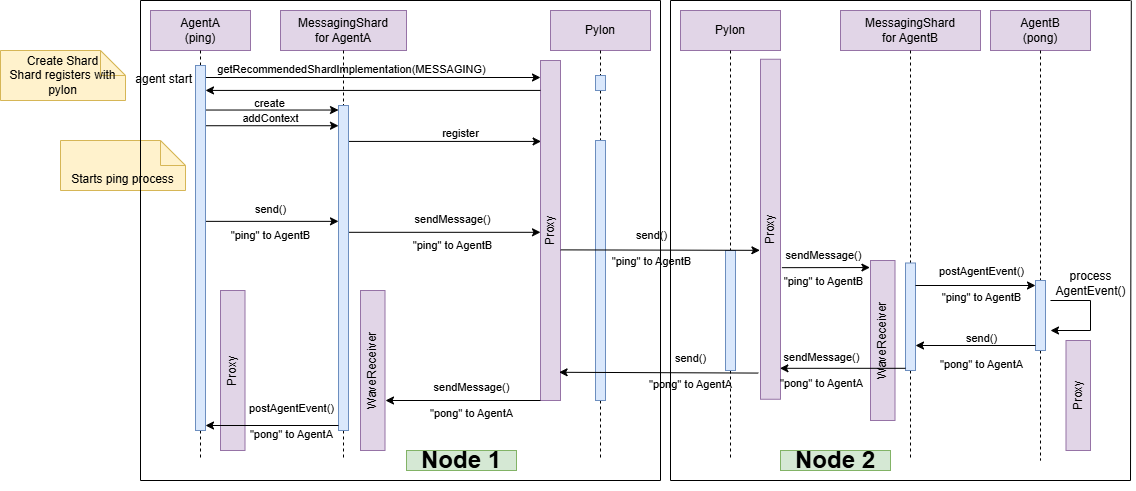
\includegraphics[scale=0.37]{../img/AgentPingPongSequenceDiagramFinal.png}
  \caption{Sequence diagram containing the agents, the pylon, and the shards.}
  \label{fig:AgentPingPongSequenceDiagramFinal}
\end{figure}

Figure~\ref{fig:ContextStructureDiagram} presents an UML class diagram for the agent - shard - pylon - pylon proxy - shard container structuring, especially from a context perspective.

\begin{figure}[t]
\centering
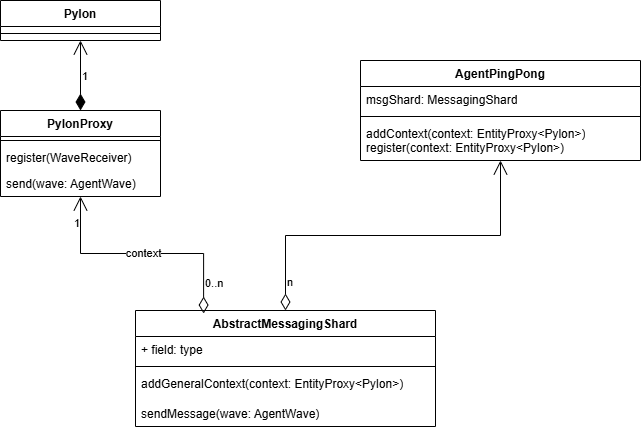
\includegraphics[scale=0.4]{../img/ContextStructureDiagram.png}
  \caption{UML class diagram for the agent - shard - pylon - pylon proxy - shard container structuring, especially from a context perspective.}
  \label{fig:ContextStructureDiagram}
\end{figure}

\subsubsection{Starting the deployment}

To start the deployment, one can run the \code{Boot} class from the \code{simplePingPong} subpackage under \code{src-examples/example}. In this file, one can select the desired interaction with the communication infrastructure, either directly using \code{AgentPingPongPlain}, or via a \code{messagingShard} by means of \code{AgentPingPong}. 

Regardless of the option, the node, the names of the agents involved, the configuration of the \code{sendTo} parameter with the names of the agents that will receive messages, as well as the number of pings sent must be provided.

\section{Maven}
\clearpage

\subsection{Build}

To build the \fmas project via Maven, one can run in the root directory of the project, the commands below.

To build the project using the integrated profile \code{build-only}, run:

\code{mvn clean install -P build-only}

To build the project using plain Maven, run:

\code{mvn clean install -DskipTests}


\subsection{Tests}

To execute the tests using the integrated profile \code{tests-only}, run:

\code{mvn test -P tests-only}


\subsection{Build and tests}

To build the project and execute the tests using plain Maven, run:

\code{mvn clean install}

\subsection{Configuration of source directories}

Source directories can be configured in \code{pom.xml} file, in the \code{build-helper-maven-plugin} by adding a new element as in figure~\ref{fig:func:source_directories_configuration:code}.

\begin{figure}[ht]\centering
\begin{lstlisting}
<configuration>
    <sources>
        <source>src</source>
        <source>src-examples</source>
        <source>src-tests</source>
        <source>src-experiments</source>
    </sources>
</configuration>
\end{lstlisting}
\caption{Configuration of source directories}\label{fig:func:source_directories_configuration:code}
\end{figure}


\subsection{Upgrade of dependencies}

The upgrade of dependencies is done in 2 ways, depending on how they were configured in \code{pom.xml}.

There are dependencies that have a BOM available, which means that in the \code{<dependencyManagement>} section in the \code{pom.xml} file, the respective BOM will be updated to the desired version, and thus all the covered dependencies will be upgraded. Such dependencies are \code{io.vertx} and \code{com.fasterxml.jackson}.
Dependencies with BOM are configured in the \code{pom.xml} file in \code{<dependencyManagement>} section.


For the other dependencies that do not have a BOM available, the upgrade is done specifically for each one.

Figure~\ref{fig:func:JavaWebSocketDependency:code} presents a dependency that do not have a BOM available. These kind of dependencies are configured in \code{<dependencies>} section. For each dependency the \code{<version>} section should be updated to include the desired version.

\begin{figure}[ht]\centering
\begin{lstlisting}
<dependency>
    <groupId>org.java-websocket</groupId>
    <artifactId>Java-WebSocket</artifactId>
     <version>1.4.0</version>
</dependency>
\end{lstlisting}
\caption{Java WebSocket dependency}\label{fig:func:JavaWebSocketDependency:code}
\end{figure}

\subsection{Generating a jar with all dependencies}

To generate a \code{.jar} with all dependencies, the \code{maven-assembly-plugin} is necessary, being present in \code{pom.xml} file. 

To generate a \code{.jar} with all dependencies, one can run in the root directory of the project, the command below. It will be generated in the \code{target} directory.

\code{mvn clean package}


\clearpage
\section{CompositeAgent}

The \code{CompositeAgent} class implements an agent formed by shards and an event queue that allows shards to communicate among each other.

The \code{CompositeAgent} has four main structural pillars.

\paragraph{The Shard Container} 

The \code{CompositeAgent} maintains a registry of its attached shards. Various agent shards(instances of \code{AgentShard}) can be added. Shards are identified by means of their designation. At most one shard with the same designation is allowed.

\paragraph{The Event System} 

The \code{CompositeAgent} utilizes an internal, thread-safe \code{eventQueue} to receive \code{AgentEvent} objects and dispatch them to the registered shards.

Figures~\ref{fig:AgentEventActivityDiagramFirstPart} and ~\ref{fig:AgentEventActivityDiagramContinuation} are diagrams that captures all the steps performed in the event processing cycle in a \code{CompositeAgent}.

\begin{figure}[t]
\centering
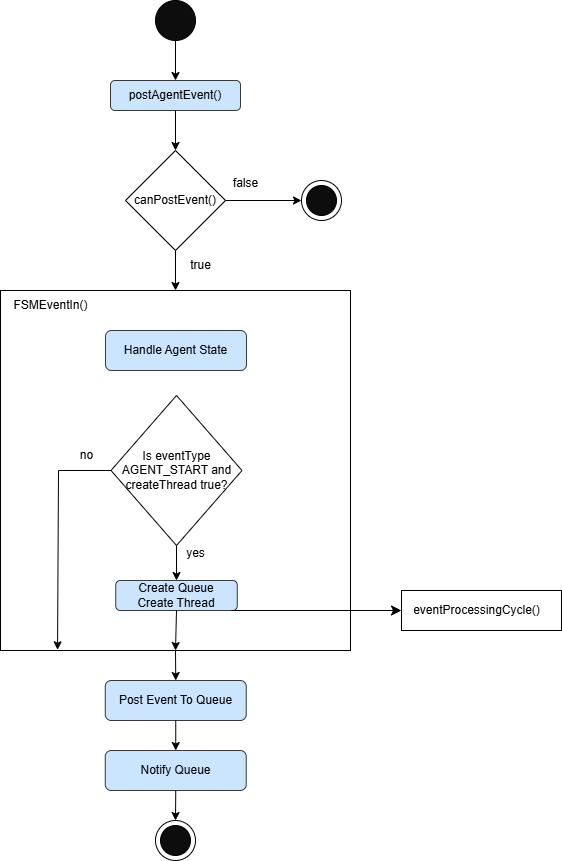
\includegraphics[scale=0.40]{../img/AgentEventActivityDiagramFirstPart.png}
  \caption{UML Activity Diagram that describes the event processing cycle in a Composite Agent (1)}
  \label{fig:AgentEventActivityDiagramFirstPart}
\end{figure}

\begin{figure}[t]
\centering
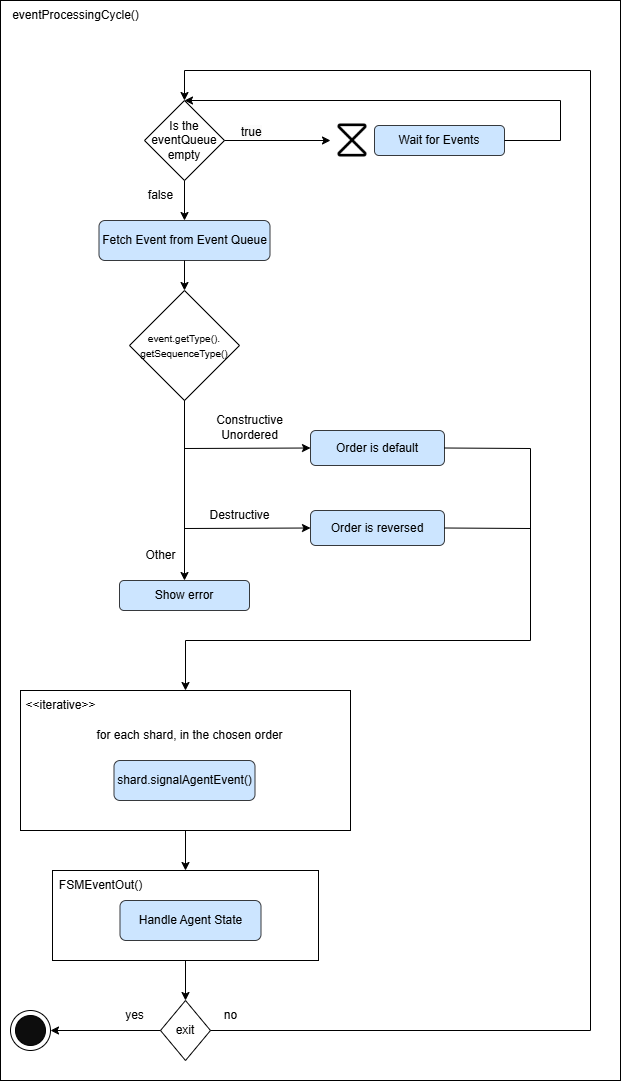
\includegraphics[scale=0.40]{../img/AgentEventActivityDiagramContinuation.png}
  \caption{UML Activity Diagram that describes the event processing cycle in a Composite Agent (2)}
  \label{fig:AgentEventActivityDiagramContinuation}
\end{figure}

\paragraph{The Dedicated Thread} 

The \code{CompositeAgent} operates on its own dedicated \code{AgentThread}. This runs a continuous event-processing loop, dequeuing and routing messages.

\paragraph{The State Machine} 

The normal transition between states is the following: \code{STOPPED} → \code{STARTING} → \code{RUNNING} → \code{STOPPING}. Additionally, it implements a \code{TRANSIENT} state. This acts as a structural freeze, locking the agent to safely allow serialization or migration across devices, preventing any shard modifications during the transition.

Figure~\ref{fig:agentStates} is an activity diagram in which the states of the \code{CompositeAgent} can be visualized, as well as the transitions between them generated by certain events.

\begin{figure}[t]
\centering
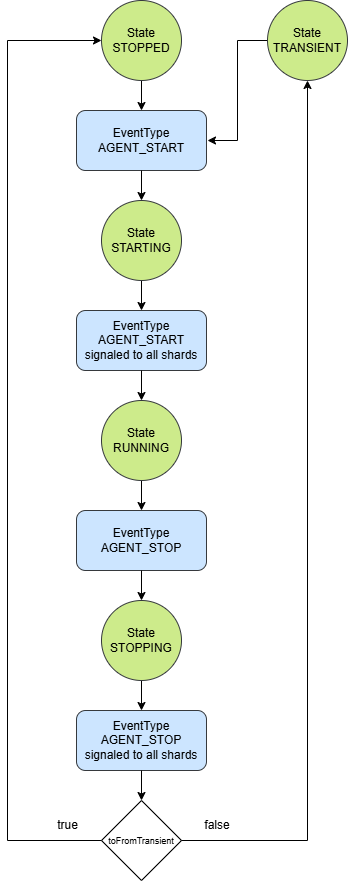
\includegraphics[scale=0.5]{../img/AgentStateActivityDiagram.png}
  \caption{UML Activity Diagram that highlights the transition between states in a Composite Agent}
  \label{fig:agentStates}
\end{figure}


\clearpage
\section{Shard}

A shard (also called a component) is characterized by its functionality, identified by means of its designation(an
instance of \code{AgentShardDesignation}).
The purpose of shards is to encapsulate specific functionality that can be used by an agent (e.g. messaging, mobility). 
An agent shard can only work as part of an agent. As such, it has access to a proxy to the agent which must be an \code{ShardContainer}.

In \fmas, agents fall into two main categories:
\begin{itemize}
    \item Composite agents: agents formed by multiple shards (components) for different functionalities
    \item Non-composite agents: simple agents that implement the \code{Agent} interface or extend \code{BaseAgent} class
\end{itemize}

To integrate a shard in a non-composite agent, one should follow these steps:
\begin{itemize}
    \item create the shard instance
    \item ask the pylon via \code{AgentShardCore.instantiateRecommendedShard()} which implementation to use
    \item pass a proxy object to comunicate with the agent via \code{postAgentEvent()}
    \item connect the shard to the pylon via \code{addGeneralContext()}
    \item notify the shard when agent starts via \code{signalAgentEvent()}
\end{itemize}

A messaging shard is a special shard that handles inter-agent communication. The messaging shard implements the \code{MessagingShard} interface and allows agents to communicate by sending \code{AgentWave} objects through a pylon.

The \code{AgentShardCore} class serves as base for the implementation of agent shards. A shard can belong to at most one \code{Agent}, which is its parent (and, in \code{Entity} terms, its context). When created, the shard has no parent; a parent will be set afterwards and the shard notified. In the life-cycle of a shard, it will be constructed and configured, then started and eventually stopped. This implementation manages the configuration of the shard and the shard's state.

The most important methods in the \code{AgentShardCore} class are
\begin{itemize}
    \item getAgent(): retrieves the parent of the shard (the \code{CompositeAgent})
    \item getShardDesignation(): returns the shard's designation
    \item configure(MultiTreeMap configuration): verify and load agent-independent shard data, based on deployment data
    \item start() and stop(): perform startup/shutdown
    \item signalAgentEvent(AgentEvent event): called by the parent when an event occurs
    \item parentChangeNotifier(ShardContainer oldParent): performs actions when the parent of the shard changes
    \item shardInitializer(): perform actions when the shard is created.
\end{itemize}

The \code{AgentShardGeneral} class extends \code{AgentShardCore}  and offers additional functionality for \code{AgentShard} implementations, especially in working together with other (known types of) shards.

The most important methods in the \code{AgentShardGeneral} class are
\begin{itemize}
    \item getAgentShard(AgentShardDesignation designation): retrieves other shards from the same agent.
    \item getMessagingShard(): retrieves the agent's messaging shard.
    \item sendMessage(): uses the \code{MessagingShard} to send a message
\end{itemize}

Figure~\ref{fig:DiagramShardLoadingVertical} is a diagram which describes the process of loading a shard.

\begin{figure}[t]
\centering
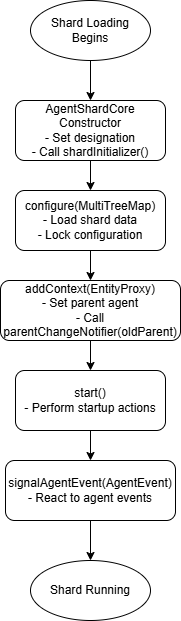
\includegraphics[scale=0.35]{../img/DiagramShardLoadingVertical.png}
  \caption{Diagram which describes the process of loading a shard}
  \label{fig:DiagramShardLoadingVertical}
\end{figure}

\clearpage
\section{Pylon}

The \code{Pylon} interface should be implemented by any persistent entity that exists on a \code{Node} and offers to agents services such as communication, mobility, or directory management. The pylon represents the local execution environment (the support infrastructure) for the agents. As a \code{ConfigurableEntity}, it also provides the \code{getSupportedServices()} method, returning the names of the services the instance supports.

\paragraph{Shard Recommendation}

In \fmas, agents are built modularly, and the appropriate shard implementation often depends heavily on the support infrastructure (e.g., local versus network messaging). To address this, the \code{Pylon} interface provides the \code{getRecommendedShardImplementation(AgentShardDesignation shardType)} method. 

Using this method, agents can be easily implemented by asking the pylon for the recommended shard class name for a specific functionality, rather than hardcoding it. 

\paragraph{DefaultPylonImplementation}

The \code{DefaultPylonImplementation} serves as the minimal base infrastructure for agents. It provides a default context management system but offers no additional services natively (returning an empty set for supported services and \code{null} for recommended shards). Both \code{LocalPylon} and \code{WebSocketPylon} extend this base class to build their specific routing logic.

\paragraph{LocalPylon}

The \code{LocalPylon} class is a simple support implementation that allows agents to send messages locally (inside the same JVM) based strictly on the agent's name. It relies on \code{AgentWave} objects for message passing.

There are two ways in which this implementation can work:
\begin{itemize}
    \item \textbf{Queued method (default)}: A separate thread is used to process a \code{LinkedBlockingQueue} to which messages are added. This is the recommended approach to avoid race conditions and deadlocks.
    \item \textbf{Direct method}: The \code{send()} method leads directly to a call of the \code{receive()} method of the shard in the destination agent. This method does not use a separate thread.
\end{itemize}

Beyond basic routing, the \code{LocalPylon} can be configured through parameters such as \code{use-thread}, \code{keep-undeliverable-for}, and \code{retry-every}. These parameters manage how the pylon handles messages whose destinations have not yet been registered, allowing it to either discard them or queue them for delayed retry.

When queried via \code{getRecommendedShardImplementation} for a messaging shard, the \code{LocalPylon} recommends the \code{SimpleLocalMessaging} class (an alias for \code{NameBasedMessagingShard}), which is optimized for in-memory communication.

% un exemplu de pylon local cu 2 agenti in el

Figure~\ref{fig:func:LocalPylon:code} presents a 
deployment configuration using \code{LocalPylon} via command line arguments.

\begin{figure}[ht]\centering
\begin{lstlisting}
-package example.localDeployment
-pylon local:default
-agent AgentOne classpath:AgentOne
-agent AgentTwo classpath:AgentTwo
\end{lstlisting}
\caption{Deployment configuration via command line arguments}\label{fig:func:LocalPylon:code}
\end{figure}

\paragraph{WebSocketPylon}

The \code{WebSocketPylon} class provides a support implementation that allows agents to communicate whether they are inside the same JVM or distributed across a network. This pylon connects to a \code{WebSocketServerEntity}. Any agent in the context of this support can send messages to agents located on any other pylon connected to the same WebSocket server.

Configuration is handled via attributes such as \code{connectTo} (the server address) or \code{serverPort}. If a port is provided, the pylon can instantiate the WebSocket server directly on the local node. When connecting as a client, it implements a resilient mechanism that will automatically attempt to reconnect multiple times if the connection fails.

The message routing and delivery process involves the following steps:
\begin{itemize}
    \item \textbf{Registration}: Entities are registered to the pylon and a JSON message (containing \code{nodeName} and \code{entityName}) is sent to the server to update the global directory. A similar process handles unregistration using an \code{unregister} key.
    \item \textbf{Local Delivery}: If the destination entity is registered locally within the pylon, the message is delivered directly to its \code{WaveReceiver}.
    \item \textbf{External Delivery}: If the destination is external, the \code{AgentWave} is serialized into a JSON object, appended with routing metadata, and sent to the server.
    \item \textbf{Incoming Messages}: JSON messages received from the server are parsed, converted back into \code{AgentWave} objects, and routed to the correct local entity.
\end{itemize}

Similar to the \code{LocalPylon}, the \code{WebSocketPylon} utilizes a message queue and a dedicated \code{MessageThread} to handle asynchronous message processing. When queried for a messaging shard recommendation, it returns the \code{WebSocketMessagingShard} class.

% un exemplu cu 2 noduri, si fiecare cu cate un websocketpylon si un agent

Figure~\ref{fig:func:WebSocketPylon:code} presents a deployment configuration using \code{WebSocketPylon} via command line arguments.

\begin{figure}[ht]\centering
\begin{lstlisting}
-package testing -loader agent:composite
-node node1
-pylon webSocket:pylon1 serverPort:8886
-agent composite:AgentA -shard messaging -shard PingTest otherAgent:AgentB -shard EchoTesting
-node node2
-pylon webSocket:pylon2 connectTo:ws://localhost:8886
-agent composite:AgentB -shard messaging -shard PingBackTest -shard EchoTesting
\end{lstlisting}
\caption{Deployment configuration via command line arguments}\label{fig:func:WebSocketPylon:code}
\end{figure}




\end{document}
